% Figure: Laplace's equation on a unit square with one inhomogeneous
% boundary. Shows the level curves of the leading-mode solution
% u(x,y) = sin(pi x) sinh(pi y) / sinh(pi) and the maximum-principle
% bound.
\begin{figure}[htbp]
\centering
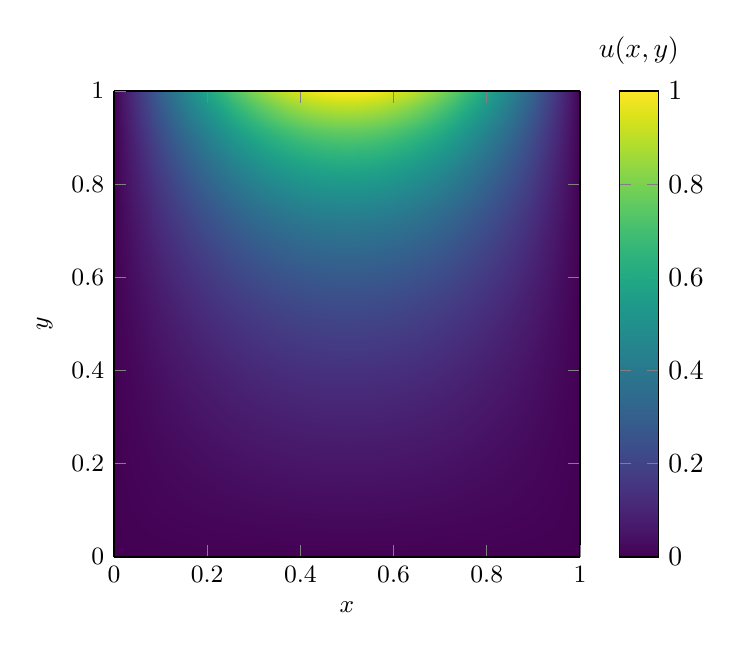
\begin{tikzpicture}
\begin{axis}[
  width=8.5cm, height=7.5cm,
  view={0}{90},
  xlabel={$x$},
  ylabel={$y$},
  xmin=0, xmax=1,
  ymin=0, ymax=1,
  axis equal image,
  colormap/viridis,
  colorbar,
  colorbar style={
    title={$u(x,y)$},
    ytick={0,0.2,0.4,0.6,0.8,1.0},
  },
  font=\small,
  point meta min=0, point meta max=1,
]
\addplot3[
  surf, shader=interp,
  samples=60, samples y=60,
  domain=0:1, y domain=0:1,
] { sin(deg(pi*x)) * sinh(pi*y) / sinh(pi) };
\end{axis}
\end{tikzpicture}
\caption[Laplace solution on a unit square]{Steady-state solution
of $\laplacian u = 0$ on the unit square with boundary data
$u(x,0) = u(0,y) = u(1,y) = 0$ and $u(x,1) = \sin(\pi x)$, obtained
by separation of variables as $u(x,y) = \sin(\pi x)\sinh(\pi
y)/\sinh(\pi)$. The colour map shows the field. The maximum
principle is satisfied: the field attains its maximum $u = 1$ on
the top boundary at $x = 1/2$, its minimum $u = 0$ on the other
three edges, and every interior value lies strictly between. The
exponential-style decay of the sinh ratio sets the penetration
depth of the boundary detail into the interior.}
\label{fig:vol02:ch12:laplace-square}
\end{figure}
